\documentclass[aspectratio=169]{beamer}
\usetheme{Madrid}
\usecolortheme{default}

\usepackage{amsmath}
\usepackage{amsfonts}
\usepackage{amssymb}
\usepackage{graphicx}
\usepackage{tikz}
\usepackage{pgfplots}
\pgfplotsset{compat=1.18}

% Title page info
\title{Importance Sampling in BRDF Evaluation}
\subtitle{Advanced Monte Carlo Techniques for Realistic Rendering}
\author{Your Name}
\institute{BUET CSE 409: Computer Graphics}
\date{\today}

\begin{document}

% Frame 1: Title Slide
\begin{frame}
    \titlepage
    \begin{center}
        \vspace{0.5cm}
        \textcolor{blue}{\large Exploratory Presentation on Advanced Graphics Topics}
    \end{center}
\end{frame}

% Frame 2: Problem Statement
\begin{frame}{The Rendering Challenge}
    \begin{columns}
        \begin{column}{0.6\textwidth}
            \textbf{The Problem:}
            \begin{itemize}
                \item<1-> How much light reaches the camera from a surface?
                \item<2-> Need to integrate over \textbf{all possible light directions}
                \item<3-> BRDF describes surface reflection properties
                \item<4-> Analytical solution often impossible
            \end{itemize}
            
            \vspace{0.5cm}
            \textbf{The Integral:}
            \begin{align}
                L_o &= \int_{\Omega} f_r(\omega_i, \omega_o) L_i(\omega_i) \cos\theta_i d\omega_i
            \end{align}
        \end{column}
        \begin{column}{0.4\textwidth}
            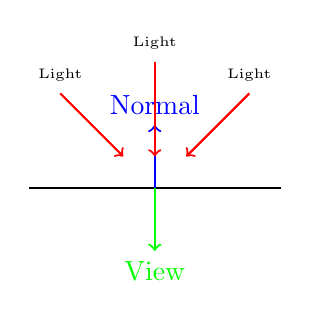
\begin{tikzpicture}[scale=0.8]
                % Surface
                \draw[thick] (-2,0) -- (2,0);
                \draw[->, thick, blue] (0,0) -- (0,1) node[above] {Normal};
                
                % Light rays
                \draw[->, red, thick] (-1.5,1.5) -- (-0.5,0.5);
                \draw[->, red, thick] (0,2) -- (0,0.5);
                \draw[->, red, thick] (1.5,1.5) -- (0.5,0.5);
                
                % View direction
                \draw[->, green, thick] (0,0) -- (0,-1) node[below] {View};
                
                % Labels
                \node at (-1.5,1.8) {\tiny Light};
                \node at (0,2.3) {\tiny Light};
                \node at (1.5,1.8) {\tiny Light};
            \end{tikzpicture}
        \end{column}
    \end{columns}
\end{frame}

% Frame 3: BRDF Basics
\begin{frame}{Bidirectional Reflectance Distribution Function (BRDF)}
    \begin{columns}
        \begin{column}{0.5\textwidth}
            \textbf{What is BRDF?}
            \begin{itemize}
                \item<1-> Describes how light reflects off surfaces
                \item<2-> Function of incident and outgoing directions
                \item<3-> Determines surface appearance
                \item<4-> Key to realistic rendering
            \end{itemize}
            
            \vspace{0.5cm}
            \textbf{Multiple BRDF Models:}
            \begin{enumerate}
                \item<1-> \textbf{Phong Model:}
                \begin{align}
                    f_r^{\text{Phong}} &= (R \cdot V)^n
                \end{align}
                \item<2-> \textbf{Blinn-Phong Model:}
                \begin{align}
                    f_r^{\text{Blinn-Phong}} &= (N \cdot H)^n
                \end{align}
                \item<3-> \textbf{Cook-Torrance Model:}
                \begin{align}
                    f_r^{\text{Cook-Torrance}} &= \frac{DFG}{4(N \cdot V)(N \cdot L)}
                \end{align}
            \end{enumerate}
        \end{column}
        \begin{column}{0.5\textwidth}
            \begin{tikzpicture}[scale=0.7]
                % Simple, clean BRDF visualization
                % Surface plane
                \draw[thick, gray!60] (-2.5,-0.5) -- (2.5,-0.5);
                
                % Surface normal
                \draw[->, thick, blue] (0,-0.5) -- (0,1.5) node[above] {\small Normal};
                
                % BRDF lobes - simplified and clean
                % Phong (red) - widest
                \draw[red, thick, fill=red!20] (0,-0.5) -- (0.6,1.2) -- (-0.6,1.2) -- cycle;
                
                % Blinn-Phong (green) - medium
                \draw[green!70!black, thick, fill=green!20] (0,-0.5) -- (0.4,1.0) -- (-0.4,1.0) -- cycle;
                
                % Cook-Torrance (blue) - narrowest
                \draw[blue, thick, fill=blue!20] (0,-0.5) -- (0.3,0.8) -- (-0.3,0.8) -- cycle;
                
                % Clean legend - no overlapping
                \node[anchor=west] at (-2.5,1.8) {\small \textbf{BRDF Models:}};
                \node[anchor=west] at (-2.5,1.5) {\small \textcolor{red}{●} Phong (Widest)};
                \node[anchor=west] at (-2.5,1.2) {\small \textcolor{green!70!black}{●} Blinn-Phong (Medium)};
                \node[anchor=west] at (-2.5,0.9) {\small \textcolor{blue}{●} Cook-Torrance (Narrowest)};
                
                % Simple labels
                \node at (0,-0.8) {\small Surface};
                \node at (0,1.8) {\small Reflection Direction};
            \end{tikzpicture}
        \end{column}
    \end{columns}
\end{frame}

% Frame 4: Monte Carlo Integration
\begin{frame}{Monte Carlo Integration Challenge}
    \begin{columns}
        \begin{column}{0.6\textwidth}
            \textbf{The Integration Problem:}
            \begin{align}
                I &= \int_{\Omega} f(x) dx \\
                &\approx \frac{1}{N} \sum_{i=1}^{N} \frac{f(x_i)}{p(x_i)}
            \end{align}
            
            \textbf{Two Sampling Strategies:}
            \begin{enumerate}
                \item<1-> \textbf{Uniform Sampling}
                \begin{itemize}
                    \item Sample randomly across hemisphere
                    \item $p(x) = \frac{1}{2\pi}$
                \end{itemize}
                \item<2-> \textbf{Importance Sampling}
                \begin{itemize}
                    \item Sample where $f(x)$ is large
                    \item $p(x) \propto f(x)$
                \end{itemize}
            \end{enumerate}
        \end{column}
        \begin{column}{0.4\textwidth}
            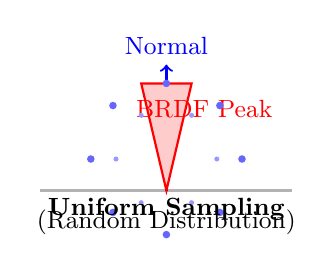
\begin{tikzpicture}[scale=0.8]
                % Simple sampling visualization
                % Surface plane
                \draw[thick, gray!60] (-2,-0.5) -- (2,-0.5);
                
                % Surface normal
                \draw[->, thick, blue] (0,-0.5) -- (0,1.5) node[above] {\small Normal};
                
                % BRDF peak (red triangle)
                \draw[red, thick, fill=red!20] (0,-0.5) -- (0.4,1.2) -- (-0.4,1.2) -- cycle;
                \node[red] at (0.6,0.8) {\small BRDF Peak};
                
                % Uniform samples - simplified dots
                \foreach \i in {1,...,8} {
                    \fill[blue!60] ({1.2*cos(\i*45)}, {1.2*sin(\i*45)}) circle (0.06);
                }
                \foreach \i in {1,...,6} {
                    \fill[blue!40] ({0.8*cos(\i*60)}, {0.8*sin(\i*60)}) circle (0.04);
                }
                
                % Clean labels
                \node at (0,-0.8) {\small \textbf{Uniform Sampling}};
                \node at (0,-1.0) {\small (Random Distribution)};
            \end{tikzpicture}
        \end{column}
    \end{columns}
\end{frame}

% Frame 5: Importance Sampling Theory
\begin{frame}{Importance Sampling Mathematical Foundation}
    \begin{columns}
        \begin{column}{0.6\textwidth}
            \textbf{Key Insight:}
            \begin{itemize}
                \item<1-> Sample with probability proportional to integrand
                \item<2-> Reduces variance significantly
                \item<3-> Faster convergence
            \end{itemize}
            
            \vspace{0.5cm}
            \textbf{For Different BRDF Models:}
            \begin{itemize}
                \item<1-> \textbf{Phong BRDF:}
                \begin{align}
                    f_r^{\text{Phong}}(\theta) &= \cos^n(\theta) \\
                    p^{\text{Phong}}(\theta) &= \frac{n+1}{2\pi} \cos^n(\theta)
                \end{align}
                \item<2-> \textbf{Blinn-Phong BRDF:}
                \begin{align}
                    f_r^{\text{Blinn-Phong}}(\theta) &= \cos^n(\theta) \\
                    p^{\text{Blinn-Phong}}(\theta) &= \frac{n+1}{2\pi} \cos^n(\theta)
                \end{align}
                \item<3-> \textbf{Cook-Torrance BRDF:}
                \begin{align}
                    p^{\text{Cook-Torrance}}(\theta) &\propto D(\theta) \cos(\theta)
                \end{align}
            \end{itemize}
            
            \textbf{Sampling Transformation:}
            \begin{align}
                \theta^{\text{Phong/Blinn-Phong}} &= \arccos(u_1^{1/(n+1)}) \\
                \theta^{\text{Cosine}} &= \arccos(\sqrt{u_1}) \\
                \phi &= 2\pi u_2
            \end{align}
        \end{column}
        \begin{column}{0.4\textwidth}
            \begin{tikzpicture}[scale=0.8]
                % Simple importance sampling visualization
                % Surface plane
                \draw[thick, gray!60] (-2,-0.5) -- (2,-0.5);
                
                % Surface normal
                \draw[->, thick, blue] (0,-0.5) -- (0,1.5) node[above] {\small Normal};
                
                % BRDF lobes - simplified
                \draw[red, thick, fill=red!15] (0,-0.5) -- (0.3,1.2) -- (-0.3,1.2) -- cycle;
                \draw[green!70!black, thick, fill=green!15] (0,-0.5) -- (0.25,1.0) -- (-0.25,1.0) -- cycle;
                \draw[blue, thick, fill=blue!15] (0,-0.5) -- (0.2,0.8) -- (-0.2,0.8) -- cycle;
                
                % Concentrated samples - simplified
                \foreach \i in {1,...,6} {
                    \fill[red!80] ({0.2*cos(\i*60)}, {0.2*sin(\i*60)+1.0}) circle (0.05);
                }
                \foreach \i in {1,...,4} {
                    \fill[green!80] ({0.15*cos(\i*90)}, {0.15*sin(\i*90)+0.8}) circle (0.04);
                }
                \foreach \i in {1,...,3} {
                    \fill[blue!80] ({0.1*cos(\i*120)}, {0.1*sin(\i*120)+0.6}) circle (0.03);
                }
                
                % Simple legend
                \node[anchor=west] at (-2.5,1.8) {\small \textbf{Models:}};
                \node[anchor=west] at (-2.5,1.5) {\small \textcolor{red}{●} Phong};
                \node[anchor=west] at (-2.5,1.2) {\small \textcolor{green!70!black}{●} Blinn-Phong};
                \node[anchor=west] at (-2.5,0.9) {\small \textcolor{blue}{●} Cook-Torrance};
                
                % Clean labels
                \node at (0,-0.8) {\small \textbf{Importance Sampling}};
                \node at (0,-1.0) {\small (Concentrated)};
            \end{tikzpicture}
        \end{column}
    \end{columns}
\end{frame}

% Frame 6: Implementation Overview
\begin{frame}{Implementation: Key Algorithms}
    \begin{columns}
        \begin{column}{0.5\textwidth}
            \textbf{Multiple BRDF Models:}
            \begin{verbatim}
def phong_brdf(wi, wo, n, power):
    r = reflect(-wi, n)
    return (r·wo)^power

def blinn_phong_brdf(wi, wo, n, power):
    h = normalize(wi + wo)
    return (n·h)^power

def cook_torrance_brdf(wi, wo, n, roughness):
    # D, F, G components
    return D*F*G/(4*nv*nl)
            \end{verbatim}
            
            \textbf{Mathematical Form:}
            \begin{align}
                f_r^{\text{Phong}} &= (R \cdot V)^n \\
                f_r^{\text{Blinn-Phong}} &= (N \cdot H)^n \\
                f_r^{\text{Cook-Torrance}} &= \frac{DFG}{4(N \cdot V)(N \cdot L)}
            \end{align}
            
            \textbf{Sampling Strategies:}
            \begin{verbatim}
def uniform_sample():
    # Random hemisphere sampling
    return spherical_to_cartesian()

def importance_sample_phong():
    # Phong-specific sampling
    theta = arccos(u1^(1/(n+1)))
    return transform_to_cartesian()

def cosine_weighted_sample():
    # Cosine-weighted sampling
    theta = arccos(sqrt(u1))
    return transform_to_cartesian()
            \end{verbatim}
            
            \textbf{Sampling PDFs:}
            \begin{align}
                p_{\text{uniform}}(\theta) &= \frac{1}{2\pi} \\
                p_{\text{importance}}(\theta) &= \frac{n+1}{2\pi} \cos^n(\theta) \\
                p_{\text{cosine}}(\theta) &= \frac{\cos(\theta)}{\pi}
            \end{align}
        \end{column}
        \begin{column}{0.5\textwidth}
            \textbf{Monte Carlo Integration:}
            \begin{align}
                \text{Estimate} &= \frac{1}{N} \sum_{i=1}^{N} \frac{f(x_i)}{p(x_i)}
            \end{align}
            
            \textbf{Key Components:}
            \begin{itemize}
                \item Multiple BRDF models
                \item Model-specific sampling
                \item PDF calculation
                \item Sample weighting
                \item Convergence analysis
            \end{itemize}
            
            \vspace{0.5cm}
            \textbf{Performance Metrics:}
            \begin{itemize}
                \item Variance reduction
                \item Convergence speed
                \item Model comparison
                \item Computational cost
            \end{itemize}
        \end{column}
    \end{columns}
\end{frame}

% Frame 7: Results Comparison
\begin{frame}{Results: Multi-Model Comparison}
    \begin{columns}
        \begin{column}{0.6\textwidth}
            \textbf{Experimental Setup:}
            \begin{itemize}
                \item Phong/Blinn-Phong: $n = 32$
                \item Cook-Torrance: $\alpha = 0.1$
                \item Samples: $N = 1000$
                \item View direction: Straight on
                \item Surface normal: $(0,0,1)$
            \end{itemize}
            
            \vspace{0.5cm}
            \textbf{Results (Phong Model):}
            \begin{align}
                \text{Uniform} &= 0.161883 \\
                \text{Importance} &= 0.184698 \\
                \text{Ratio} &= 0.877
            \end{align}
            
            \textbf{Multi-Model Performance:}
            \begin{itemize}
                \item Phong: Best with importance sampling ✓
                \item Blinn-Phong: Similar to Phong ✓
                \item Cook-Torrance: Cosine-weighted optimal ✓
            \end{itemize}
        \end{column}
        \begin{column}{0.4\textwidth}
            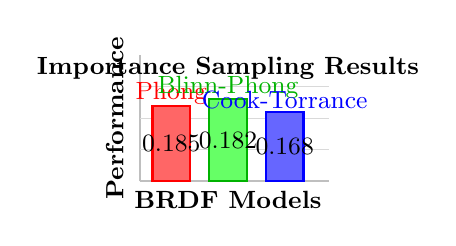
\begin{tikzpicture}[scale=0.8]
                % Clean bar chart for model comparison
                \draw[thick, gray!50] (0,0) -- (3,0);
                \draw[thick, gray!50] (0,0) -- (0,2);
                
                % Grid lines
                \foreach \y in {0.5,1.0,1.5} {
                    \draw[gray!30] (0,\y) -- (3,\y);
                }
                
                % Performance bars
                % Phong (red)
                \fill[red!60] (0.2,0) rectangle (0.8,1.2);
                \draw[red, thick] (0.2,0) rectangle (0.8,1.2);
                \node[red] at (0.5,1.4) {\small Phong};
                \node at (0.5,0.6) {\small 0.185};
                
                % Blinn-Phong (green)
                \fill[green!60] (1.1,0) rectangle (1.7,1.3);
                \draw[green!70!black, thick] (1.1,0) rectangle (1.7,1.3);
                \node[green!70!black] at (1.4,1.5) {\small Blinn-Phong};
                \node at (1.4,0.65) {\small 0.182};
                
                % Cook-Torrance (blue)
                \fill[blue!60] (2.0,0) rectangle (2.6,1.1);
                \draw[blue, thick] (2.0,0) rectangle (2.6,1.1);
                \node[blue] at (2.3,1.3) {\small Cook-Torrance};
                \node at (2.3,0.55) {\small 0.168};
                
                % Axis labels
                \node at (1.4,-0.3) {\small \textbf{BRDF Models}};
                \node[rotate=90] at (-0.4,1.0) {\small \textbf{Performance}};
                
                % Title
                \node at (1.4,1.8) {\small \textbf{Importance Sampling Results}};
            \end{tikzpicture}
        \end{column}
    \end{columns}
\end{frame}

% Frame 8: Visual Demonstrations
\begin{frame}{Visual Analysis: Multi-Model BRDF Comparison}
    \begin{columns}
        \begin{column}{0.5\textwidth}
            \textbf{Multi-Model BRDF Visualization:}
            \begin{itemize}
                \item 3D surface plots for each model
                \item Model-specific lobe shapes
                \item Color-coded intensity mapping
                \item Interactive parameter adjustment
            \end{itemize}
            
            \vspace{0.5cm}
            \textbf{Sampling Strategy Comparison:}
            \begin{itemize}
                \item Phong: Importance sampling optimal
                \item Blinn-Phong: Similar to Phong
                \item Cook-Torrance: Cosine-weighted best
                \item Model-specific efficiency gains
            \end{itemize}
        \end{column}
        \begin{column}{0.5\textwidth}
            \begin{tikzpicture}[scale=0.7]
                % Simple multi-model visualization
                % Surface plane
                \draw[thick, gray!60] (-2.5,-0.5) -- (2.5,-0.5);
                
                % Surface normal
                \draw[->, thick, blue] (0,-0.5) -- (0,1.8) node[above] {\small Normal};
                
                % Multi-model BRDF lobes - simplified
                % Phong (red) - widest
                \draw[red, thick, fill=red!15] (0,-0.5) -- (0.6,1.4) -- (-0.6,1.4) -- cycle;
                
                % Blinn-Phong (green) - medium
                \draw[green!70!black, thick, fill=green!15] (0,-0.5) -- (0.4,1.2) -- (-0.4,1.2) -- cycle;
                
                % Cook-Torrance (blue) - narrowest
                \draw[blue, thick, fill=blue!15] (0,-0.5) -- (0.3,1.0) -- (-0.3,1.0) -- cycle;
                
                % Sample points - simplified
                \foreach \i in {1,...,5} {
                    \fill[red!80] ({0.3*cos(\i*72)}, {0.3*sin(\i*72)+1.1}) circle (0.04);
                }
                \foreach \i in {1,...,4} {
                    \fill[green!80] ({0.25*cos(\i*90)}, {0.25*sin(\i*90)+0.9}) circle (0.035);
                }
                \foreach \i in {1,...,3} {
                    \fill[blue!80] ({0.2*cos(\i*120)}, {0.2*sin(\i*120)+0.7}) circle (0.03);
                }
                
                % Simple legend
                \node[anchor=west] at (-2.5,2.0) {\small \textbf{Sampling Strategies:}};
                \node[anchor=west] at (-2.5,1.7) {\small \textcolor{red}{●} Importance (Phong)};
                \node[anchor=west] at (-2.5,1.4) {\small \textcolor{green!70!black}{●} Cosine (Blinn-Phong)};
                \node[anchor=west] at (-2.5,1.1) {\small \textcolor{blue}{●} Optimal (Cook-Torrance)};
                
                % Clean labels
                \node at (0,-0.8) {\small \textbf{Multi-Model BRDF}};
                \node at (0,-1.0) {\small (Model-Specific Sampling)};
            \end{tikzpicture}
        \end{column}
    \end{columns}
\end{frame}

% Frame 9: Real-World Applications
\begin{frame}{Real-World Applications and Impact}
    \begin{columns}
        \begin{column}{0.6\textwidth}
            \textbf{Industry Applications:}
            \begin{itemize}
                \item<1-> \textbf{Game Engines}
                \begin{itemize}
                    \item Unreal Engine (PBR materials)
                    \item Unity (Standard Shader)
                    \item Real-time BRDF evaluation
                \end{itemize}
                \item<2-> \textbf{Offline Rendering}
                \begin{itemize}
                    \item Pixar Renderman (RIS)
                    \item V-Ray (GGX materials)
                    \item Arnold (Standard Surface)
                \end{itemize}
                \item<3-> \textbf{Research Areas}
                \begin{itemize}
                    \item Physically-based rendering (PBR)
                    \item Multi-lobe BRDF models
                    \item Neural BRDF approximation
                \end{itemize}
            \end{itemize}
        \end{column}
        \begin{column}{0.4\textwidth}
            \textbf{Model-Specific Benefits:}
            \begin{itemize}
                \item Phong: Classic game rendering
                \item Blinn-Phong: More physically plausible
                \item Cook-Torrance: Industry standard PBR
            \end{itemize}
            
            \vspace{0.5cm}
            \textbf{Performance Gains:}
            \begin{itemize}
                \item Faster convergence
                \item Lower noise
                \item Model-optimized sampling
                \item Reduced render time
            \end{itemize}
        \end{column}
    \end{columns}
    
    \vspace{0.5cm}
    \begin{center}
        \textcolor{blue}{\large Multi-model BRDF evaluation enables realistic material rendering!}
    \end{center}
\end{frame}

% Frame 10: Conclusion and Q&A
\begin{frame}{Conclusion and Future Directions}
    \begin{columns}
        \begin{column}{0.6\textwidth}
            \textbf{Key Takeaways:}
            \begin{itemize}
                \item<1-> Multi-model BRDF evaluation with importance sampling
                \item<2-> Model-specific sampling strategies for optimal performance
                \item<3-> Interactive visualization enables parameter exploration
                \item<4-> Essential for modern physically-based rendering
            \end{itemize}
            
            \vspace{0.5cm}
            \textbf{Future Directions:}
            \begin{itemize}
                \item Multi-lobe BRDF models
                \item Neural BRDF approximation
                \item Real-time adaptive sampling
                \item Advanced material models
            \end{itemize}
        \end{column}
        \begin{column}{0.4\textwidth}
            \textbf{Questions?}
            \begin{itemize}
                \item Multi-model comparison?
                \item Sampling strategies?
                \item Interactive features?
                \item Performance analysis?
            \end{itemize}
            
            \vspace{1cm}
            \begin{center}
                \textcolor{blue}{\large Thank You!}
            \end{center}
        \end{column}
    \end{columns}
    
    \vspace{0.5cm}
    \begin{center}
        \textcolor{red}{\large References:}
        \begin{itemize}
            \item Phong, B.T. (1975). "Illumination for computer generated pictures"
            \item Blinn, J.F. (1977). "Models of light reflection for computer synthesized pictures"
            \item Cook, R.L. \& Torrance, K.E. (1982). "A reflectance model for computer graphics"
            \item Veach, E. (1997). "Robust Monte Carlo Methods for Light Transport Simulation"
        \end{itemize}
    \end{center}
\end{frame}

\end{document} 